\documentclass[xcolor=dvipsnames, professionalfont]{beamer}

\usepackage{xcolor}
%\usepackage{tikz}

\usefonttheme{serif}

\usetheme{Berlin}
\usecolortheme[named=purple]{structure}

\author{Ali Abolhassanzadeh Mahani}
\title{Growing Critical: Self-Organized Criticality in a Developing Neural System}
\date{}
\institute{Sharif University of Technology}


\begin{document}
	\frame{\maketitle}
	\section*{Introduction}
	\begin{frame}
		{\centering
		An article by:\\
		Felipe Yaroslav Kalle Kossio, Sven Goedeke, Benjamin van
		den Akker, Borja Ibarz, and Raoul-Martin Memmesheimer
	}
		
		\begin{itemize}
			\item Intro to criticality 
			\pause
			\item Genetic development of neural networks:\\
			active neurons shrink while inactive ones grow
		\end{itemize}
	\end{frame}

	\subsection*{A bit of history}
	\begin{frame}
		
	\end{frame}

	\section*{Stationary State Dynamics}
	\begin{frame}
		The dynamics is an inhomogeneous Poisson point process (?)\\
		Notation: 
		\begin{itemize}
			\item $f_i(t)$: instantaneous firing rate of neuron $i$
			\item $gA_{ij}$: time-dependent connection strength
			\item $g$: proportionality constant
			\item $A_{ij}$: overlap areas of the neurons
			\item $\tau$: the decay time constant due to leak currents
			\item $\hat{t}_j$: spike times of neuron $j$
		\end{itemize}
	\pause
	The Stationary State Dynamics is a follows:
	\begin{equation}
		\tau \dot{f}_i(t) = f_0 - f_i(t) + \tau g \sum_j A_{ij}(t^-) \sum_{\hat{t}_j} \delta(t - \hat{t}_j)
	\end{equation}
	\end{frame}

	\section*{Network Growth}
	\begin{frame}
		Notation:
		\begin{itemize}
			\item $R_i(t)$: radius of disk representing a single neuron
			\item $K$: linear growth rate of neurons
			\item $\frac{K}{f_{sat}}$: neuron radii shrinkage at spike sending
			\item Growth takes much longer than decay of
activity $\frac{1}{K} \gg \tau$,
			\item experiments $\Rightarrow f_{sat} \gg f_0$
		\end{itemize}
	\pause
	The network growth dynamics is as follows:
	\begin{equation}
		\dot{R}_i(t) = K \left( 1 - \frac{1}{f_{sat}} \sum_{\hat{t}_i} \delta(t - \hat{t}_i) \right)
	\end{equation}
	\end{frame}
	
	\begin{frame}
		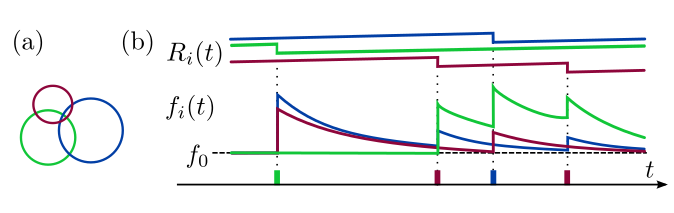
\includegraphics[width=\linewidth]{img/example.png}
		Example of the network dynamics.
	\end{frame}
	
	\section{Results}
	\begin{frame}
		Averaged over the randomness of spike generation, each spike generates in total 
		\begin{equation}
			\sigma = \tau g \sum_j \bar{A_{ij}} = 1 - \frac{f_{0}}{f_{sat}}
		\end{equation}
	spikes.
	
	Thus we have a age-dependent branching process with branching parameter $\sigma$.  (Individuals --spikes-- generate offspring at an age-dependent rate) 
	
	\textbf{Ref:} Crump-Mode-Jagers branching process
	
	\end{frame}

	\begin{frame}
	\centering
	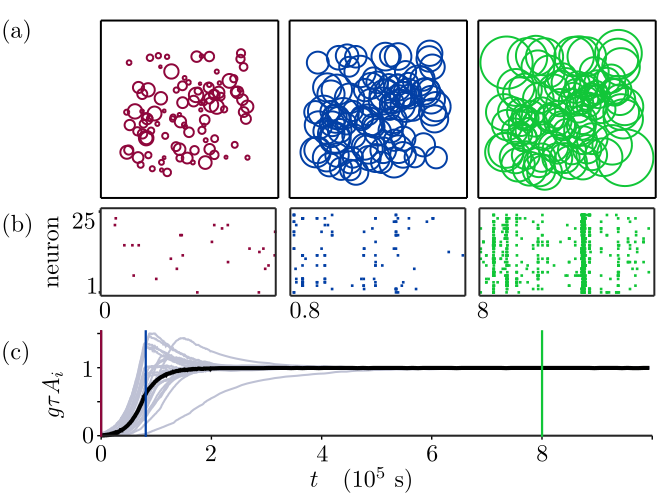
\includegraphics[width=.8\linewidth]{img/simulation.png}
	
\end{frame}

	\begin{frame}
			The avalanche sizes $s$ follow the Borel distribution 
		\begin{equation}
			P(s) = \frac{(s\sigma)^{s-1} e^{-s\sigma}}{s!}
		\end{equation}
	where using the Stirling's approximation we get
	\begin{equation}
		P_{appr}(s) = \frac{1}{\sqrt{2\pi}\sigma} s^{-\frac{3}{2}} e^{-(\sigma - \ln \sigma - 1)s}
	\end{equation}
	\pause
	
	\textbf{Notice} the power-law tail with exponent $\frac{3}{2}$ of a critical branching process for $\sigma = 1$
	\end{frame}

	\begin{frame}
		\centering
		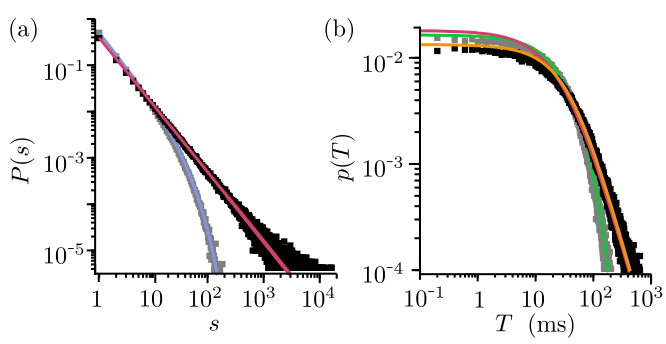
\includegraphics[width=\linewidth]{img/avalanches.png}
	\end{frame}

	\begin{frame}
		\centering
		\Large
		Thank you for your time :)
	\end{frame}
	
	
\end{document}